\documentclass[10pt, t]{beamer}
% \usepackage[UTF8]{ctex}
\usepackage{amsmath}
\usepackage{setspace}
\usepackage{float} 
\usepackage{multido}
\usepackage{multirow}
\usepackage{array}
\usepackage{enumerate}
\usepackage{booktabs}
\usepackage{indentfirst} 
\usepackage[style=mla]{biblatex}
\usepackage{setspace}
\usepackage{subcaption}
\usepackage{hyperref}
\usepackage{textpos}

\makeatletter
\let\@@magyar@captionfix\relax
\makeatother

\definecolor{bladerunnerblue}{RGB}{41, 159, 163}
\definecolor{bladerunnerred}{RGB}{194,84,97}
\definecolor{themecolor}{RGB}{25,25,112} 
\definecolor{weak}{RGB}{150,150,150}

\renewcommand{\emph}[1]{{\color{bladerunnerblue}\textsl{#1}}}
\newcommand{\alarm}[1]{{\color{bladerunnerred}{#1}}}
\newcommand{\N}{\mathbb{N}}
\newcommand{\R}{\mathbb{R}}
\newcommand{\myseries}[2]{$#1_1,#1_2,\dots,#1_#2$}
\newcommand{\nullspace}{~\\[15pt]}
\newcommand{\remark}{\textbf{Remark: }}
\newcommand{\scp}[2]{\langle\,#1\,,\,#2\,\rangle} \newcommand{\scpp}{\langle\,\cdot\,,\,\cdot\,\rangle}
\newcommand{\weaken}[1]{{\color{weak}\textit{#1}}}
\newcommand{\underover}[3]{\underset{#2}{\overset{#3}{#1}}}
\renewcommand{\emptyset}{\varnothing}


\usetheme{Madrid}
\setbeamertemplate{navigation symbols}{}

\addtobeamertemplate{frametitle}{}{
\begin{textblock*}{100mm}(0.85\textwidth,-1cm)
\includegraphics[height=1cm]{../../logo.png}
\end{textblock*}}


\usecolortheme[named=themecolor]{structure}

\setbeamertemplate{items}[default]

\hypersetup{
    colorlinks=true,
    linkcolor=themecolor,
    filecolor=themecolor,      
    urlcolor=themecolor,
    citecolor=themecolor,
}

\title{VV186: Honors Mathematics}
\subtitle{\large Math Foundations}
\institute[UM-SJTU JI]{Univerity of Michigan-Shanghai Jiao Tong University Joint Institute}
\author{Xingjian Zhang}

\begin{document}

\begin{frame}
    \titlepage
    \begin{center}
        \includegraphics[height=2cm]{../../logo2.png}
    \end{center}
\end{frame}

\begin{frame}
    \frametitle{About Exam}
    \begin{itemize}
        \item 30 pts, possibly contain
        \begin{enumerate}
        \item Multiple choice questions (The choices can be all wrong.)
        \item Calculation question
        \item Proof question 
        \item Explanation question
        \item \dots
        \end{enumerate}
        \item 100 mins
        \item 100/30 = 3.3 mins/pt. Therefore, you probably don't want to spend more than 5 mins on 1 pt.
        \item Don't panic if you cannot figure out all some specific question. Just skip it and do it later.
        \item The questions may not be arranged in the order of difficulty.
    \end{itemize}
\end{frame}

\begin{frame}
    \frametitle{Checking List}
    \begin{itemize}
        \item Truth Table
        \item Prove by Contraposition
        \item Logical/Sets Operation
        \item Properties of Natural/Rational/Complex Numbers
        \item \textbf{Mathematical Induction}
    \end{itemize}
    Part 0 is \textbf{not} the key point of the exam. However, you should still go through these concepts. Though they might not be directly tested, they could occur somewhere in your exam paper.
\end{frame}

\begin{frame}
    \frametitle{Truth Table}
    \begin{figure}[H]
        \centering
        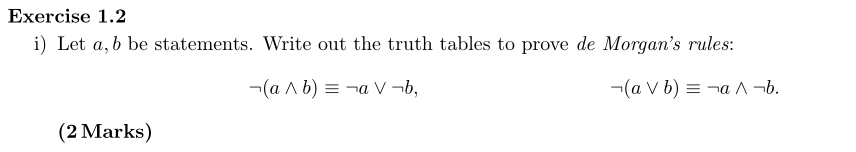
\includegraphics[width=\textwidth]{2020-10-17-23-11-31.png}
    \end{figure}

    Notice that the last column of the truth table should be an evaluation on equivalence. For example, for the first question, you should evaluate $\neg(a \wedge b)\Leftrightarrow \neg a \vee \neg b$. It is supposed to be true for the whole column. Only through this fact can you conclude that $\neg(a \wedge b)\equiv \neg a \vee \neg b$.\nullspace
    Please distinguish equivalence ($\Leftrightarrow$) and logical equivalence ($\equiv$). The former one is a binary operation, while the later one indicates a relationship between two compound statements. To be more precise, logical equivalence indicates that the equivalence between two compound statements is a tautology.

\end{frame}

\begin{frame}
    \frametitle{Contraposition}

    The famous tautology
    $$(A \Rightarrow B) \equiv(\neg B \Rightarrow \neg A)$$ is useful in some situation. If you are asked to prove some statement $A\Rightarrow B$ but you cannot find a simple way, you can try to prove by contraposition.

\end{frame}

\begin{frame}
    \frametitle{Exercise}

    Let $x \in \mathbb{Z} .$ If $x^{2}-6 x+5$ is even, then $x$ is odd.\nullspace\pause
    \textbf{Proof:} 
    Suppose that $x$ is even. Then we want to show that $x^{2}-6 x+5$ is odd. Write $x=2 a$ for some $a \in \mathbb{Z},$ and plug in:
    $$
        \begin{aligned}
            x^{2}-6 x+5 & =(2 a)^{2}-6(2 a)+5            \\
                        & =4 a^{2}-12 a+5                \\
                        & =2\left(2 a^{2}-6 a+2\right)+1
        \end{aligned}
    $$
    Thus $x^{2}-6 x+5$ is odd.

\end{frame}

\begin{frame}
    \frametitle{Mathematical Induction}

    \begin{figure}[H]
        \centering
        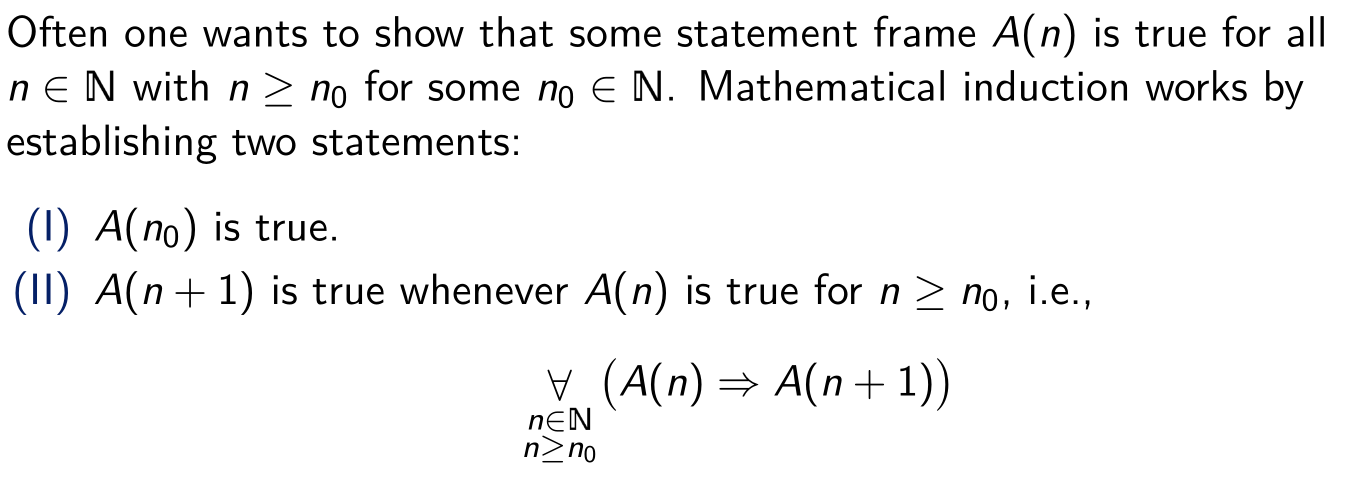
\includegraphics[width=0.9\textwidth]{2020-09-23-12-37-23.png}
    \end{figure}

    \textbf{Remark:} Mathematical Induction is basically the only relatively important concept in Part 0 of VV186. Please see Ex5, Ex6 and Ex7 in sample exam and see the related rubric.

\end{frame}

\begin{frame}
    \frametitle{Exercises}
    Let $a_{n}$ be the following expression with $n$ nested radicals:
    $$
        a_{n}=\sqrt{2+\sqrt{2+\cdots+\sqrt{2+\sqrt{2}}}}
    $$
    Prove that $a_{n}=2 \cos \frac{\pi}{2^{n+1}}$


\end{frame}

\begin{frame}
    \frametitle{Exercise}
    \textbf{Proof: }Note that $a_{n}$ can be defined recursively like this: $a_{1}=\sqrt{2},$ and $a_{n+1}=\sqrt{2+a_{n}}$ for $n \geq 1 .$ We proceed by induction. For $n=1$ we have in fact $a_{1}=\sqrt{2},$ and $2 \cos \frac{\pi}{4}=2 \cdot \frac{1}{\sqrt{2}}=\sqrt{2}$.\nullspace
    Next, assuming the result is true for some $n \geq 1,$ we have
    $$
        \begin{aligned}
            a_{n+1} & =\sqrt{2+a_{n}}=\sqrt{2+2 \cos \frac{\pi}{2^{n+1}}}       \\
                    & =\sqrt{2+2 \cos 2 \frac{\pi}{2^{n+2}}}                    \\
                    & =\sqrt{2+2\left(2 \cos ^{2} \frac{\pi}{2^{n+2}}-1\right)} \\
                    & =\sqrt{4 \cos ^{2} \frac{\pi}{2^{n+2}}}                   \\
                    & =2 \cos \frac{\pi}{2^{n+2}}
        \end{aligned}
    $$
    By induction, we conclude that $a_{n}=2 \cos \frac{\pi}{2^{n+1}}$.
\end{frame}

\begin{frame}
    \frametitle{Exercise}

    We define recursively the \textit{Ulam} numbers by setting $u_{1}=1, u_{2}=2,$ and for each subsequent integer $n,$ we set $n$ equal to the next \textit{Ulam} number if it can be written uniquely as the sum of two different \textit{Ulam} numbers; e.g.: $u_{3}=3, u_{4}=4, u_{5}=6,$ etc. Prove that there are infinitely many \textit{Ulam} numbers.

\end{frame}

\begin{frame}
    \frametitle{Exercise}

    \textbf{Proof: } \nullspace
    We prove there are infinitely many \textit{Ulam} numbers by induction.\nullspace
    For $n=1,2$, $u_1=1,\, u_2=2$ are defined. \nullspace
    Next, we assume if we have found the first $m\geq 2$ \textit{Ulam} numbers, we can always find $u_{m+1}$ that satisfy the recursive definition. Let $U_{m}=\left\{u_{1}, u_{2}, \ldots, u_{m}\right\}(m \geq 2)$ be the first $m$ \textit{Ulam} numbers (written in increasing order $) .$ Let $S_{m}$ be the set of integers greater than $u_{m}$ that can be written uniquely as the sum of two different Ulam numbers from $U_{m} .$ The next Ulam number $u_{m+1}$ is precisely the minimum element of $S_{m},$ unless $S_{m}$ is empty, but it is not because $u_{m-1}+u_{m} \in S_{m}$.

\end{frame}

\begin{frame}
    \frametitle{End}
    \vspace{2.2cm}
    \begin{center}
        \Large
        Good Luck!
    \end{center}
\end{frame}


\end{document}